\begin{figure}
	\centering
	\subfigure[$\Delta t$ = 1 día]{
	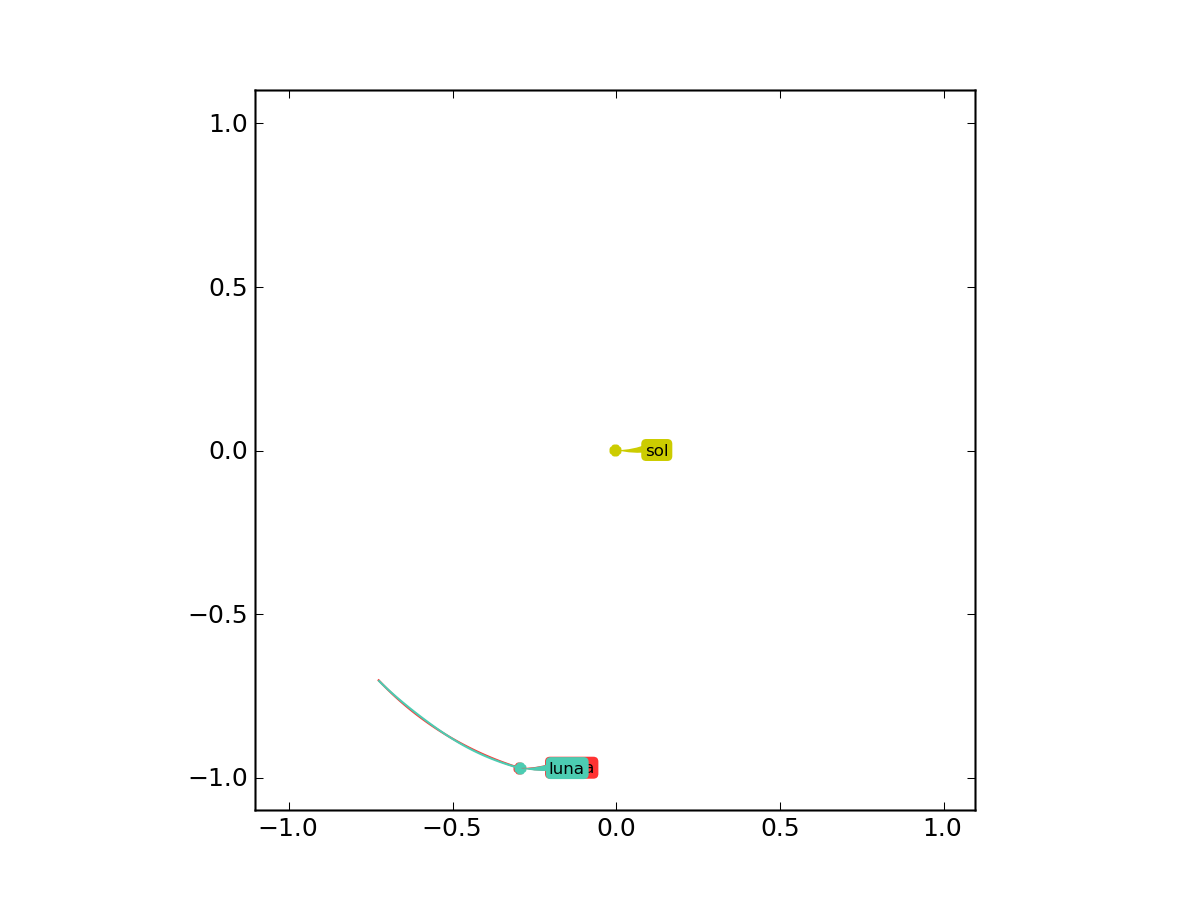
\includegraphics[scale=0.38]{img/ej1/metodo3/validacion_30_1000.png}
	\label{fig:ej1_m3_30_001}
	}
	\\
	\subfigure[$\Delta t$ = 2 horas]{
	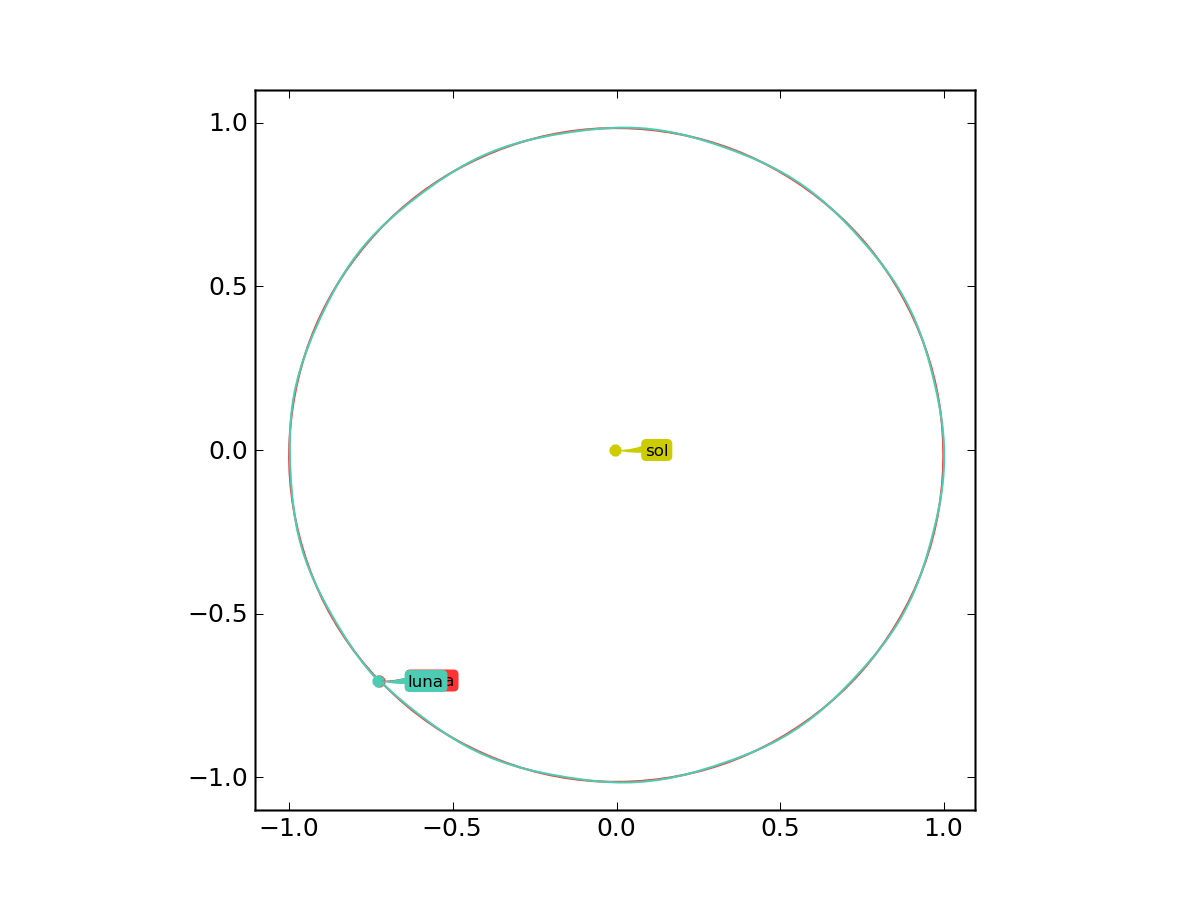
\includegraphics[scale=0.38]{img/ej1/metodo3/validacion_365_1000.png}
	\label{fig:ej1_m3_365_1000}
	}
	\subfigure[$\Delta t$ = 1 hora]{
	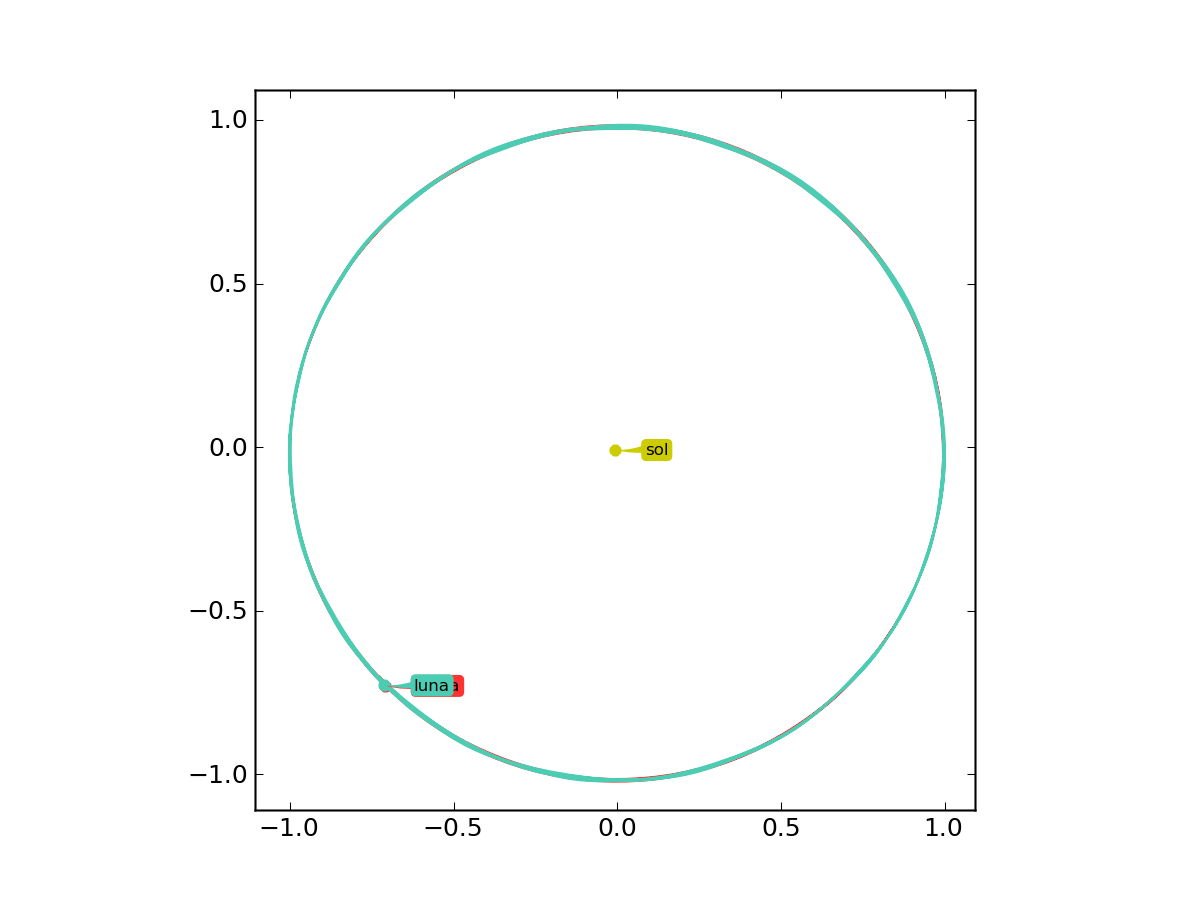
\includegraphics[scale=0.38]{img/ej1/metodo3/validacion_1825_1000.png}
	\label{fig:ej1_m3_1825_1000}
	}
	\caption{
		Simulación de validación del sistema sol$-$tierra$-$luna distintos períodos y un $\Delta t$ de $1/1000$ días
		con el método 3. El método solo funciona bien con $\Delta t$ de este órden o mas chicos.
		Al intentar validar para los $\Delta t$ usados en los otros métodos, no obteníamos resultados razonables.
	}
	\label{ fig:res_ej1_m3 }
\end{figure}
